% +------------------------------------------------------------------------+
% | CGAL Reference Manual:  polyhedron.tex
% +------------------------------------------------------------------------+
% | Combinatoric and geometry of polyhedral surfaces in 
% | halfedge representation.
% |
% | 11.10.1996   Lutz Kettner
% |              Start rewriting the whole stuff
% | 
\RCSdef{\polyhedronRev}{$Revision$}
\RCSdefDate{\polyhedronDate}{$Date$}
% +------------------------------------------------------------------------+

\ccParDims

\chapter{3D Polyhedral Surfaces}
\label{chapterPolyhedron}
\ccChapterRelease{\polyhedronRev. \ \polyhedronDate}\\
\ccChapterAuthor{Lutz Kettner}

\vspace*{-15mm}
\minitoc
\vspace*{30mm}

% +------------------------------------------------------------------------+
\section{Release Note}

\begin{ccTexOnly}
    \vspace*{-50mm}
    \begin{flushright}~\hspace{1cm}
      \parbox{0.5\textwidth}{%
          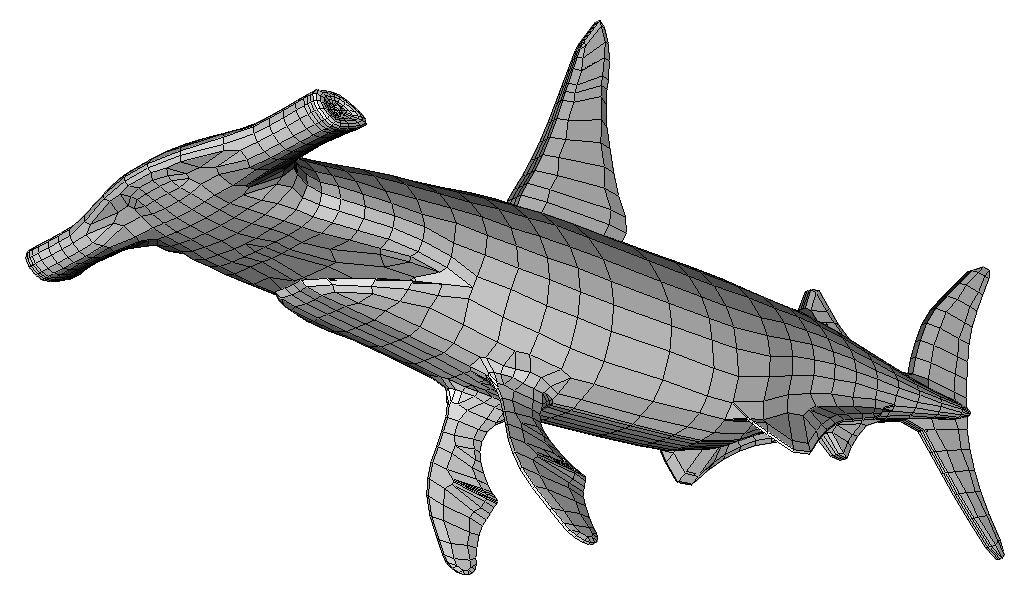
\includegraphics[width=0.5\textwidth]{fig/shark.ps}%
      }%
    \end{flushright}
\end{ccTexOnly}

Beginning with \cgal\ R2.3, this package has a new design.  The old
design is still available for backwards compatibility and to support
older compiler, such as MSVC++6.0. However its use is deprecated and
the manual pages are not converted into this new manual
format. Instead, see its old documentation in the manual of 
deprecated packages.

For the polyhedral surface, old and new design cannot be used
simultaneously (they have identical include file names and class
names). The include files select automatically the old design for
MSVC++6.0 and the new design otherwise. This automatism can be
overwritten by defining appropriate macros before the include
files. The old design is selected with the 
\texttt{CGAL\_USE\_POLYHEDRON\_DESIGN\_ONE} macro. The new design 
is selected with the 
\texttt{CGAL\_USE\_POLYHEDRON\_DESIGN\_TWO} macro.

The new design differs from the old design in the following ways: The
\ccc{Polyhedron_3} has a different number of template parameters that
require different concepts, such as the new \ccc{HalfedgeDS} concept,
the new \ccc{PolyhedronItems_3} concept, and the new
\ccc{PolyhedronTraits_3} concept. The \ccc{Polyhedron_3} interface is
backwards compatible with the old design except that the
\ccc{normal()} member function in the facet and related types disappear.
Please use the plane equation instead, see also
\ccc{Polyhedron_traits_with_normals_3} in the reference manual.

% +------------------------------------------------------------------------+
\section{Introduction}
\label{sectionPolyIntro}

Polyhedral surfaces in three dimensions are composed of vertices,
edges, facets and an incidence relationship on them. The organization
beneath is a halfedge data structure, which restricts the class of
representable surfaces to orientable 2-manifolds -- with and without
boundary. If the surface is closed we call it a {\em polyhedron}, for
example, see the \ccTexHtml{above}{following} model of a hammerhead:

\begin{ccHtmlOnly}
    <CENTER>
        <img src="./shark.gif" alt="Hammerhead"><P>
    </CENTER>
\end{ccHtmlOnly}

The polyhedral surface is realized as a container class that manages
vertices, halfedges, facets with their incidences, and that maintains
the combinatorial integrity of them. It is based on the highly
flexible design of the halfedge data structure, see the introduction
in Chapter~\ref{chapterHalfedgeDS} and~\cite{k-ugpdd-99}. However, the
polyhedral surface can be used and understood without knowing the
underlying design. Some of the examples in this chapter introduce also
gradually into first applications of this flexibility.

% +========================================================================+
\section{Definition}
% +========================================================================+
  
A polyhedral surface \ccc{CGAL::Polyhedron_3<PolyhedronTraits_3>} in
three dimensions consists of vertices $V$, edges $E$, facets $F$ and
an incidence relation on them.  Each edge is represented by two
halfedges with opposite orientations. The incidences stored with a
halfedge are illustrated in the following figure:

\begin{ccTexOnly}
    \vspace{-7mm}
    \begin{center}
      \parbox{0.4\textwidth}{%
          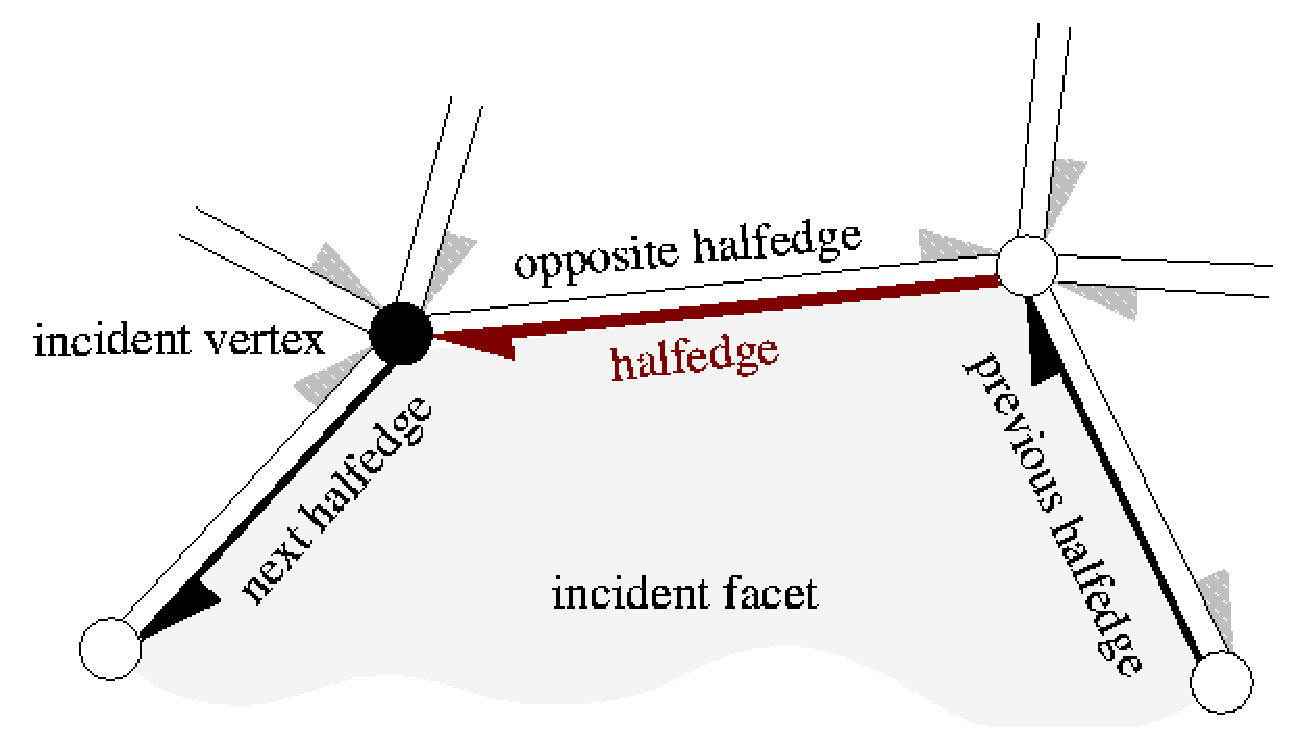
\includegraphics[width=0.4\textwidth]{fig/halfedge.ips}%
      }
    \end{center}
    \vspace{-5mm}
\end{ccTexOnly}

\begin{ccHtmlOnly}
    <CENTER>
    <A HREF="./halfedge.gif">
        <img src="./halfedge_small.gif" alt="Halfedge Diagram"></A><P>
    </CENTER>
\end{ccHtmlOnly}

Vertices represent points in space. Edges are straight line segments
between two endpoints. Facets are planar polygons without
holes. Facets are defined by the circular sequence of halfedges along
their boundary.  The polyhedral surface itself can have holes (with at
least two facets surrounding it since a single facet cannot have a
hole). The halfedges along the boundary of a hole are called {\em
border halfedges\/} and have no incident facet. An edge is a {\em
border edge\/} if one of its halfedges is a border halfedge.  A
surface is {\em closed\/} if it contains no border halfedges. A closed
surface is a boundary representation for polyhedra in three
dimensions. The convention is that the halfedges are oriented
counterclockwise around facets as seen from the outside of the
polyhedron. An implication is that the halfedges are oriented
clockwise around the vertices. The notion of the solid side of a facet
as defined by the halfedge orientation extends to polyhedral surfaces
with border edges although they do not define a closed object. If
normal vectors are considered for the facets, normals point outwards
(following the right-hand rule).

The strict definition can be found in~\cite{k-ugpdd-99}. One
implication of this definition is that the polyhedral surface is
always an orientable and oriented 2-manifold with border edges, i.e.,
the neighborhood of each point on the polyhedral surface is either
homeomorphic to a disc or to a half disc, except for vertices where
many holes and surfaces with boundary can join. Another implication is
that the smallest representable surface avoiding self intersections is
a triangle (for polyhedral surfaces with border edges) or a
tetrahedron (for polyhedra). Boundary representations of orientable
2-manifolds are closed under Euler operations. They are extended with
operations that create or close holes in the surface.

Other intersections besides the incidence relation are not allowed.
However, this is not automatically verified in the operations, since
self intersections are not easy to check
efficiently. \ccc{CGAL::Polyhedron_3<PolyhedronTraits_3>} does only
maintain the combinatorial integrity of the polyhedral surface (using
Euler operations) and does not consider the coordinates of the points
or any other geometric information.

\ccc{CGAL::Polyhedron_3<PolyhedronTraits_3>} can represent polyhedral
surfaces as well as polyhedra. The interface is designed in such a way
that it is easy to ignore border edges and work only with polyhedra.


% +========================================================================+
\section{Example Programs}
% +========================================================================+
\label{sectionPolyExamples}

The polyhedral surface is based on the highly flexible design of the
halfedge data structure. Examples for this flexibility can be found in
Section~\ref{sectionPolyExtend} and in Section~\ref{sectionHdsExamples}. 
This design is not a prerequisite to understand the following examples.
See also the Section~\ref{sectionPolyAdvanced} below for some advanced 
examples.

% +-------------------------------------------------------------+
\subsection{First Example Using Defaults}

The first example instantiates a polyhedron using a kernel as traits
class. It creates a tetrahedron and stores the reference to one of its
halfedges in a \ccc{Halfedge_handle}. Handles, also know as
{\em trivial iterators}, are used to keep references to halfedges,
vertices, or facets for future use. There is also a \ccc{Halfedge_iterator}
type for enumerating halfedges. Such an iterator type can be used 
wherever a handle is required. Respective \ccc{Halfedge_const_handle} and
\ccc{Halfedge_const_iterator} for a constant polyhedron and similar
handles and iterators with \ccc{Vertex_} and \ccc{Facet_} prefix
are provided too.

The example continues with a test if the halfedge
actually refers to a tetrahedron. This test checks the connected 
component referred to by the halfedge \ccc{h} and not the polyhedral
surface as a whole. This examples works only on the combinatorial
level of a polyhedral surface. The next example adds the geometry.

\ccIncludeExampleCode{Polyhedron/polyhedron_prog_simple.C}

% +-------------------------------------------------------------+
\subsection{Example with Geometry in Vertices}

We add geometry to the our construction of a tetrahedron. Four points
are passed as arguments to the construction. This example demonstrates
in addition the use of the vertex iterator and the access to the point
in the vertices. Note the natural access notation \ccc{v->point()}.
Similarly, all information stored in a vertex, halfedge, and facet can
be accessed with a member function given a handle or iterator. For
example, given a halfedge handle \ccc{h} we can write \ccc{h->next()}
to get a halfedge handle to the next halfedge, \ccc{h->opposite()} for
the opposite halfedge, \ccc{h->vertex()} for the incident vertex at
the tip of \ccc{h}, and so on.  The output of the program will be
``\verb|1 0 0\n0 1 0\n0 0 1\n0 0 0\n|''.

%\newpage
\ccIncludeExampleCode{Polyhedron/polyhedron_prog_tetra.C}

The polyhedron offers a point iterator for convenience. The above
\texttt{for} loop simplifies to a single statement by using
\ccc{std::copy} and the ostream iterator adaptor.

\begin{ccExampleCode}
std::copy( P.points_begin(), P.points_end(), 
           std::ostream_iterator<Point_3>(std::cout,"\n"));
\end{ccExampleCode}

% +-------------------------------------------------------------+
\subsection{Example for Affine Transformation}

An affine transformation $A$ can act as a functor transforming points
and a point iterator is conveniently defined for polyhedral surfaces.
So, assuming we want only the point coordinates of a polyhedron $P$
transformed, \ccc{std::transform} does the job in a single line.

\begin{ccExampleCode}
std::transform( P.points_begin(), P.points_end(), P.points_begin(), A);
\end{ccExampleCode}


% +-------------------------------------------------------------+
\subsection{Example Computing Plane Equations}

The polyhedral surface has already provisions to store a plane
equation for each facet. However, it does not provide a function to
compute plane equations.

This example computes the plane equations of a polyhedral surface.
The actual computation is implemented in the
\texttt{compute\_plane\_equations} function.  Depending on the arithmetic
(exact/inexact) and the shape of the facets (convex/non-convex)
different methods are useful. We assume here strictly convex facets
and exact arithmetic. In our example a homogeneous representation with
\texttt{int} coordinates is sufficient. The four plane equations of the
tetrahedron are the output of the program.

\ccIncludeExampleCode{Polyhedron/polyhedron_prog_planes.C}

% +-------------------------------------------------------------+
\subsection{Example with a Vector Instead of a List Representation}
\label{sectionPolyVector}

The polyhedron class template has actually four parameters, where
three of them have default values. Using the default values explicitly
in our examples above for three parameter---ignoring the fourth
parameter, which would be a standard allocator for container class---
the definition of a polyhedron looks like:

\begin{ccExampleCode}
typedef CGAL::Polyhedron_3< Traits, 
                            CGAL::Polyhedron_items_3, 
                            CGAL::HalfedgeDS_default>      Polyhedron;
\end{ccExampleCode}

The \ccc{CGAL::Polyhedron_items_3} class contains the types used for
vertices, edges, and facets. The \ccc{CGAL::HalfedgeDS_default} class
defines the halfedge data structure used, which is a list-based
representation in this case. An alternative is a vector-based
representation. Using a vector provides random
access for the elements in the polyhedral surface and is more space
efficient, but elements cannot be deleted arbitrarily. Using a list
allows arbitrary deletions, but provides only bidirectional iterators
and is less space efficient. The following example creates again a 
tetrahedron with given points, but in a vector-based representation.

The vector-based representation resizes automatically if the reserved
capacity is not sufficient for the new items created. Upon resizing
all handles, iterators, and circulators become invalid. Their correct
update in the halfedge data structure is costly, thus it is advisable
to reserve enough space in advance as indicated with the alternative
constructor in the comment. 

\begin{ccAdvanced}
Note that the polyhedron and not the underlying halfedge data
structure triggers the resize operation, since the resize operation
requires some preconditions, such as valid incidences, to be fulfilled
that only the polyhedron can guarantee.
\end{ccAdvanced}

\ccIncludeExampleCode{Polyhedron/polyhedron_prog_vector.C}


% +-------------------------------------------------------------+
\subsection{Example with Circulator Writing Object File Format (OFF)}

We create a tetrahedron and write it to \ccc{std::cout} using the
Object File Format (OFF)~\cite{p-gmgv15-94}.  This example makes use
of \stl\ algorithms (\ccc{std::copy}, \ccc{std::distance}), \stl\
\ccc{std::ostream_iterator}, and \cgal\ circulators. The polyhedral
surface provides convenient circulators for the counterclockwise
circular sequence of halfedges around a facet and the clockwise
circular sequence of halfedges around a vertex.

However, the computation of the vertex index in the inner loop of the
facet output is not advisable with the \ccc{std::distance} function,
since it takes linear time for non random-access iterators, which
leads to quadratic runtime. For better runtime the vertex index needs
to be stored separately and computed once before writing the
facets. It can be stored, for example, in the vertex itself or in a
hash-structure.  See also the following Section~\ref{sectionPolyIO} for 
file I/O.

\ccIncludeExampleCode{Polyhedron/polyhedron_prog_off.C}

% +-------------------------------------------------------------+
\subsection{Example Using Euler Operators to Build a Cube}

Euler operators are the natural way of modifying polyhedral surfaces.
We provide a set of operations for polyhedra: \ccc{split_facet()}, 
\ccc{join_facet()}, \ccc{split_vertex()}, \ccc{join_vertex()},
\ccc{split_loop()}, and \ccc{join_loop()}. We add further convenient
operators, such as \ccc{split_edge()}. However, they could be implemented 
using the six operators above. Furthermore, we provide more operators
to work with polyhedral surfaces with border edges, for example, creating
and deleting holes. We refere to the references manual for the 
definition and illustratives figures of the Euler operators.

The following example implements a function that appends a unit cube
to a polyhedral surface. To keep track of the different steps during
the creation of the cube a sequence of sketches might help with labels
for the different handles that occur in the program code. The following
Figure shows six selected steps from the creation sequence. These steps 
are also marked in the program code.

\begin{ccTexOnly}
    \begin{center}
      \parbox{\textwidth}{%
          \includegraphics[width=\textwidth]{fig/make_cube.ips}%
      }
    \end{center}
\end{ccTexOnly}

\begin{ccHtmlOnly}
    <CENTER>
        <img src="./make_cube.gif" alt="Steps in making a cube."><P>
    </CENTER>
\end{ccHtmlOnly}


\ccIncludeExampleCode{Polyhedron/polyhedron_prog_cube.C}



% +========================================================================+
\section{File I/O}
% +========================================================================+
\label{sectionPolyIO}

Simple file I/O for polyhedral surfaces is already provided in the
library. The file I/O considers so far only the topology of the
surface and its point coordinates. It ignores a possible plane
equation or any user-added attributes, such as color.

The default file format supported in \cgal\ for output as well as for
input is the Object File Format, OFF, with file extension {\tt .off},
which is also understood by GeomView~\cite{p-gmgv15-94}. For OFF
an ASCII and a binary format exist. The format can be selected with
the \cgal\ modifiers for streams, \ccc{set_ascii_mode} and
\ccc{set_binary_mode} respectively. The modifier \ccc{set_pretty_mode}
can be used to allow for (a few) structuring comments in the
output. Otherwise, the output would be free of comments.  The default
for writing is ASCII without comments. Both, ASCII and binary format,
can be read independent of the stream setting. Since this file format
is the default format, iostream operators are provided for it.

\ccThree{Inventor_ostream&M}{}{.}
\ccInclude{CGAL/IO/Polyhedron_iostream.h}

\ccHtmlNoLinks
\ccGlobalFunction{template <class PolyhedronTraits_3>
    ostream& operator<<( ostream& out, 
                         const CGAL::Polyhedron_3<PolyhedronTraits_3>& P);}

\ccHtmlNoLinks
\ccGlobalFunction{template <class PolyhedronTraits_3>
    istream& operator>>( istream& in, 
                         CGAL::Polyhedron_3<PolyhedronTraits_3>& P);}


Additional formats supported for writing are OpenInventor ({\tt .iv})
\cite{w-impoo-94}, VRML 1.0 and 2.0 ({\tt .wrl})
\cite{bpp-vrml-95,vrmls-96,hw-vrml2h-96}, and Wavefront Advanced
Visualizer object format ({\tt .obj}). Another convenient output
function writes a polyhedral surface to a GeomView process spawned
from the \cgal\ program.  These output functions are provided as
stream operators, now acting on the stream type of the respective
format.

\ccInclude{CGAL/IO/Inventor_ostream.h}
\\
\ccInclude{CGAL/IO/VRML_1_ostream.h}
\\
\ccInclude{CGAL/IO/VRML_2_ostream.h}
\\
\ccInclude{CGAL/IO/Geomview_stream.h}

\ccHtmlNoLinks
\ccGlobalFunction{template <class PolyhedronTraits_3>
    Inventor_ostream& operator<<( Inventor_ostream& out, 
                           const CGAL::Polyhedron_3<PolyhedronTraits_3>& P);}

\ccHtmlNoLinks
\ccGlobalFunction{template <class PolyhedronTraits_3>
    VRML_1_ostream& operator<<( VRML_1_ostream& out, 
                           const CGAL::Polyhedron_3<PolyhedronTraits_3>& P);}

\ccHtmlNoLinks
\ccGlobalFunction{template <class PolyhedronTraits_3>
    VRML_2_ostream& operator<<( VRML_2_ostream& out, 
                           const CGAL::Polyhedron_3<PolyhedronTraits_3>& P);}

\ccHtmlNoLinks
\ccGlobalFunction{template <class PolyhedronTraits_3>
    Geomview_stream& operator<<( Geomview_stream& out, 
                           const CGAL::Polyhedron_3<PolyhedronTraits_3>& P);}


All these file formats have in common that they represent a surface as
a set of facets. Each facet is a list of indices pointing into a set
of vertices. Vertices are represented as coordinate triples. The
file I/O for polyhedral surfaces \ccc{CGAL::Polyhedron_3} imposes certain 
restrictions on these formats. They must represent a permissible 
polyhedral surface, e.g., a 2-manifold and no isolated vertices, see 
Section~\ref{sectionPolyIntro}.

Some example programs around the different file formats are provided
in the distribution under \texttt{examples/Polyhedron\_IO/} and
\texttt{demo/Polyhedron\_IO/}.


% +========================================================================+
\section{Extending Vertices, Halfedges, and Facets}
% +========================================================================+
\label{sectionPolyExtend}

In Section~\ref{sectionPolyVector} we have seen how to change the 
default list representation

\begin{ccExampleCode}
typedef CGAL::Polyhedron_3< Traits, 
                            CGAL::Polyhedron_items_3, 
                            CGAL::HalfedgeDS_default>      Polyhedron;
\end{ccExampleCode}

to a vector based representation of the underlying halfedge data
structure. Now we want to look a bit closer at the second template argument,
\texttt{Polyhedron\_items\_3}, that specifies what kind of vertex, 
halfedge, and facet is used. The implementation of 
\texttt{Polyhedron\_items\_3} looks a bit involved with nested 
wrapper class templates. But ignoring this technicality, what remains
are three local typedefs that define the \texttt{Vertex}, the
\texttt{Halfedge}, and the \texttt{Face} for the polyhedral surface.
Note that we use here \texttt{Face} instead of facet. Face is the term
used for the halfedge data structure. Only the top layer of the
polyhedral surface gives alias names renaming face to facet.

\begin{ccExampleCode}
class Polyhedron_items_3 {
public:
    template < class Refs, class Traits>
    struct Vertex_wrapper {
        typedef typename Traits::Point_3 Point;
        typedef CGAL::HalfedgeDS_vertex_base<Refs, CGAL::Tag_true, Point> Vertex;
    };
    template < class Refs, class Traits>
    struct Halfedge_wrapper {
        typedef CGAL::HalfedgeDS_halfedge_base<Refs>                      Halfedge;
    };
    template < class Refs, class Traits>
    struct Face_wrapper {
        typedef typename Traits::Plane_3 Plane;
        typedef CGAL::HalfedgeDS_face_base<Refs, CGAL::Tag_true, Plane>   Face;
    };
};
\end{ccExampleCode}

If we look up in the reference manual the definitions of the three
classes used in the typedefs, we will see the confirmation that the
default polyhedron uses all supported incidences, a point in the
vertex class, and a plane equation in the face class. Note how the
wrapper class provides two template parameters, \texttt{Refs}, which
we discuss a bit later, and \texttt{Traits}, which is the geometric
traits class used by the polyhedral surface and which provides us here
with the types for the point and the plane equation.

Using this example code we can write our own items class. Instead, we
illustrate an easier way if we only want to exchange one class. We use
a simpler face without the plane equation but with a color attribute
added. To simplify the creation of a vertex, halfedge, or face class,
it is always recommended to derive from one of the given base classes.
Even if the base class would contain no data it would provide
convenient type definitions. So, we derive from the base class, repeat
the mandatory constructors if necessary---which is not the case for
faces but would be for vertices---and add the color attribute.

\begin{ccExampleCode}
template <class Refs>
struct My_face : public CGAL::HalfedgeDS_face_base<Refs> {
    CGAL::Color color;
};
\end{ccExampleCode}

The new items class is derived from the old items class and the
wrapper containing the face typedef gets overridden. Note that the
name of the wrapper and its template parameters are fixed. They cannot
be changed even if, as in this example, a template parameter is not
used.

\begin{ccExampleCode}
struct My_items : public CGAL::Polyhedron_items_3 {
    template <class Refs, class Traits>
    struct Face_wrapper {
        typedef My_face<Refs> Face;
    };
};
\end{ccExampleCode}

When we use our new items class with the polyhedral surface, our new
face class is used in the halfedge data structure and the color
attribute is available in the type \texttt{Polyhedron::Facet}. However,
\texttt{Polyhedron::Facet} is not the same type as our local face 
typedef for \texttt{My\_face}, but it is derived therefrom. Thus,
everything that we put in the local face type except constructors is
then available in the \texttt{Polyhedron::Facet} type. For more
details, see the Chapter~\ref{chapterHalfedgeDS} on the halfedge data
structure design.

Pulling all pieces together, the full example program illustrates how easy
the color attribute can be accessed once it is defined.

\ccIncludeExampleCode{Polyhedron/polyhedron_prog_color.C}

We come back to the first template parameter, \texttt{Refs}, of the
wrapper classes. This parameter provides us with local types that
allow us to make further references between vertices, halfedges, and
facets, which have not already been prepared for in the current
design. These local types are \texttt{Vertex\_handle},
\texttt{Halfedge\_handle}, \texttt{Face\_handle}, and there respective
\texttt{\ldots\_const\_handle}. We add now a new vertex reference to a
face class as follows. Encapsulation and access functions could be
added for a more thorough design, but we omit that here for the sake
of brevity. The integration of the face class with the items class
works as illustrated above.

\begin{ccExampleCode}
template <class Refs>
struct My_face : public CGAL::HalfedgeDS_face_base<Refs> {
    typedef typename Refs::Vertex_handle Vertex_handle;
    Vertex_handle vertex_ref;
};
\end{ccExampleCode}

More advanced examples can be found in the Section~\ref{sectionHdsExamples}
illustrating further the design of the halfedge data structure.


% +========================================================================+
\section{Advanced Example Programs}
% +========================================================================+
\label{sectionPolyAdvanced}

% +------------------------------------------------------------------------+
\subsection{Example Creating a Subdivision Surface}

This program reads a polyhedral surface from the standard input and
writes a refined polyhedral surface to the standard output. Input and
output are in the Object File Format, OFF, with the common file
extension {\tt .off}, which is also understood by
GeomView~\cite{p-gmgv15-94}.

The refinement is a single step of the $\sqrt{3}$-scheme for creating
a subdivision surface~\cite{k-s-00}. Each step subdivides a facet
into triangles around a new center vertex, smoothes the position of the
old vertices, and flips the old edges. The program is organized along
this outline. In each of these parts, the program efficiently uses the
knowledge that the newly created vertices, edges, and facets have been
added to the end of the sequences. The program needs additional
processing memory only for the smoothing step of the old vertices.

\begin{ccTexOnly}
    \begin{center}
      \parbox{\textwidth}{%
          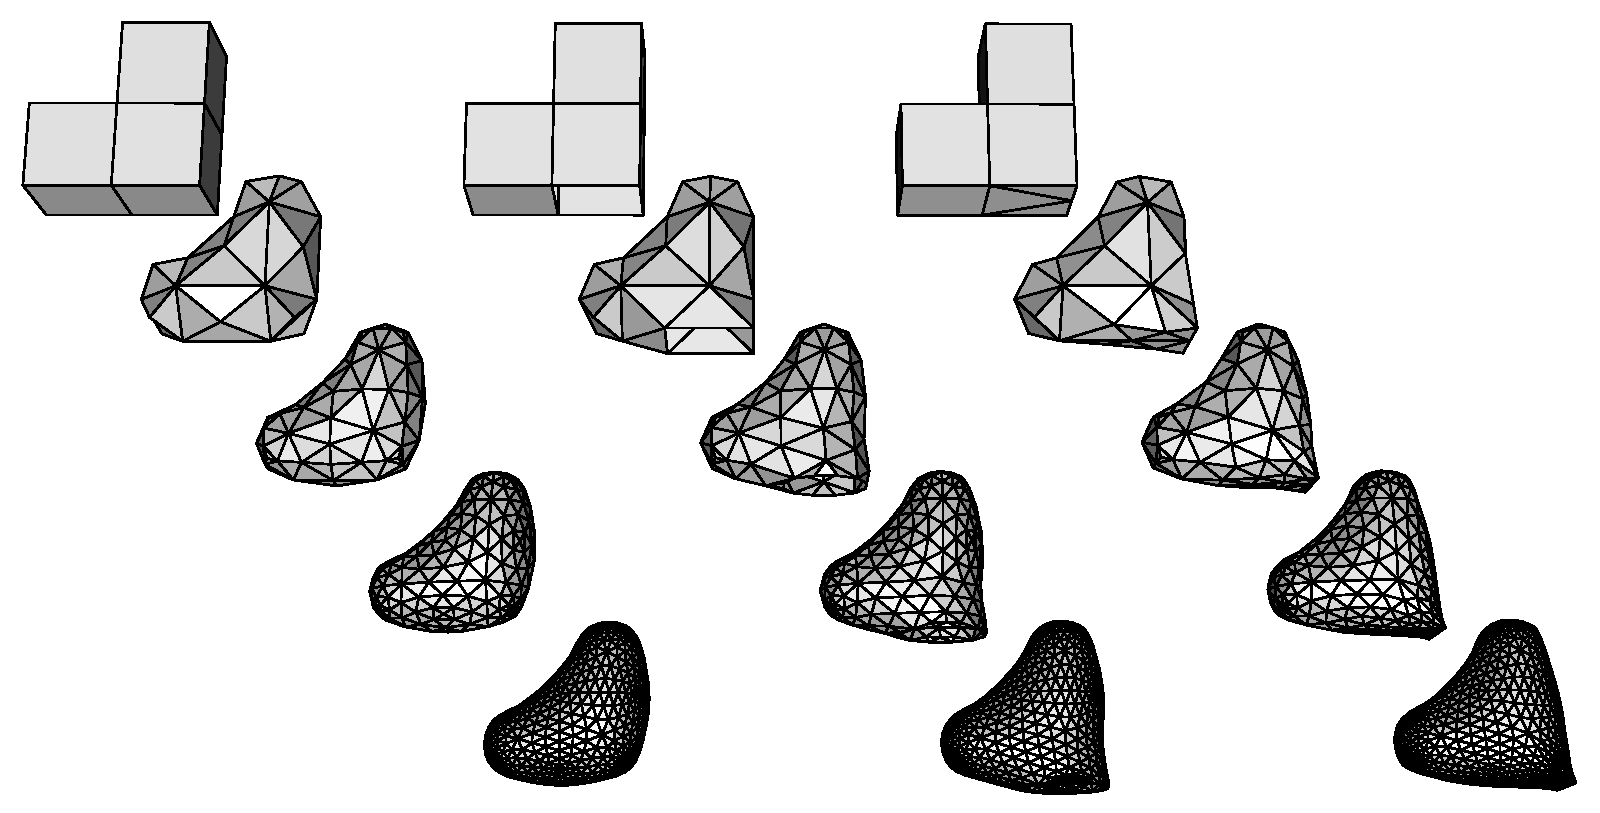
\includegraphics[width=\textwidth]{fig/subdiv.ps}%
      }
    \end{center}
\end{ccTexOnly}

\begin{ccHtmlOnly}
    <CENTER>
        <A HREF="./subdiv.gif">
            <img src="./subdiv_small.gif" alt="subdivision examples">
        </A><P>
    </CENTER>
\end{ccHtmlOnly}

The above figure shows three example objects, each 
subdivided four times. The initial object for the left sequence is
the closed surface of three unit cubes glued together to a corner.
The example program shown here can handle only closed surfaces, 
but the extended example
\texttt{examples/Polyhedron/polyhedron\_prog\_subdiv\_with\_boundary.C}
handles surfaces with boundary. So, the middle sequence starts with
the same surface where one of the facets has been removed. The boundary
subdivides to a nice circle. The third sequence creates a sharp
edge using a trick in the object presentation. The sharp edge is 
actually a hole whose vertex coordinates pinch the hole shut to form an
edge. The example directory \texttt{examples/Polyhedron/} contains the 
OFF files used here.

\ccIncludeExampleCode{Polyhedron/polyhedron_prog_subdiv.C}

% +------------------------------------------------------------------------+
\subsection{Example Using the Incremental Builder and Modifier Mechanism}

A utility class \ccc{CGAL::Polyhedron_incremental_builder_3} helps in
creating polyhedral surfaces from a list of points followed by a list
of facets that are represented as indices into the point list. This is
particularly useful for implementing file reader for common file
formats.  It is used here to create a triangle.

A modifier mechanism allows to access the internal representation of
the polyhedral surface, i.e., the halfedge data structure, in a
controlled manner. A modifier is basically a callback mechanism using
a function object. When called, the function object receives the
internal halfedge data structure as a parameter and can modify it.  On
return, the polyhedron can check the halfedge data structure for
validity. Such a modifier object must always return with a halfedge
data structure that is a valid polyhedral surface. The validity check is
implemented as an expensive postcondition at the end of the \ccc{delegate()}
member function, i.e., it is not called by default, only when expensive
checks are activated.

In this example, \ccc{Build_triangle} is such a function object
derived from \ccc{CGAL::Modifier_base<HalfedgeDS>}. The \ccc{delegate()}
member function of the polyhedron accepts this function object and calls
its \ccc{operator()} with a reference to its internally used halfedge 
data structure. Thus, this member function in \ccc{Build_triangle} can 
create the triangle in the halfedge data structure.

\ccIncludeExampleCode{Polyhedron/polyhedron_prog_incr_builder.C}

% +--------------------------------------------------------+

%% % =============================================================================
% The CGAL Reference Manual
% Chapter: Geometric Optimisation
% -----------------------------------------------------------------------------
% file   : doc_tex/basic/Optimisation/Optimisation_ref/main.tex
% package: Optimisation_doc
% author : Sven Sch�nherr <sven@inf.ethz.ch>
% -----------------------------------------------------------------------------
% $Revision$
% $Date$
% =============================================================================

\section{Reference Pages}

% =============================================================================
% The CGAL Reference Manual
% Chapter: Geometric Optimisation
% -----------------------------------------------------------------------------
% file   : doc_tex/basic/Optimisation/Optimisation_ref/reference_part.tex
% package: Optimisation_doc
% author : Sven Sch�nherr <sven@inf.ethz.ch>
% -----------------------------------------------------------------------------
% $Revision$
% $Date$
% =============================================================================

\newcommand{\inputOpt}[1]{\input{Optimisation_ref/#1.tex}}

\newcommand{\linebreakByHand}{\ccTexHtml{\linebreak[4]}{}}
\newcommand{  \newlineByHand}{\ccTexHtml{\\}{}}

% cross references
\index{minimum enclosing|see{{smallest enclosing}}}
\index{minimum spanning|see{{smallest enclosing}}}
\index{concentric spheres|see{{annulus}}}

% -----------------------------------------------------------------------------
\section*{Introduction}

This chapter describes concepts, classes, and functions for solving
geometric optimisation problems. They are divided into four categories.

\paragraph{Bounding Areas and Volumes.}
Smallest enclosing circle and ellipse (2D), smallest enclosing rectangle,
parallelogram, and strip (2D), rectangular $p$-center (2D), smallest
enclosing sphere and annulus (dD).

\paragraph{Inscribed Areas.}
Maximum area and perimeter inscribed $k$-gon (2D), extremal inscribed
$k$-gon (2D).

\paragraph{Optimal Distances.}
All furthest neigbors (2D), width of point set (3D), polytope distance (dD).

\paragraph{Advanced Techniques.}
Monotone and sorted matrix search.

\section*{Assertions}
The optimisation code uses infix \ccc{OPTIMISATION} in the assertions,
e.g.\ defining the compiler flag
\ccc{CGAL_OPTIMISATION_NO_PRECONDITIONS} switches precondition
checking off, cf.~\cgalReferToAssertions


% -----------------------------------------------------------------------------
\subsection*{Bounding Areas and Volumes}

\ccRefIdfierPage{CGAL::Min_circle_2<Traits>}\\[1ex]
\ccRefIdfierPage{CGAL::Min_circle_2_traits_2<K>}\\[1ex]
\ccRefConceptPage{MinCircle2Traits}

\smallskip

\ccRefIdfierPage{CGAL::Min_ellipse_2<Traits>}\\[1ex]
\ccRefIdfierPage{CGAL::Min_ellipse_2_traits_2<K>}\\[1ex]
\ccRefConceptPage{MinEllipse2Traits}

\smallskip

\ccRefIdfierPage{CGAL::min_rectangle_2}\\
\ccRefIdfierPage{CGAL::min_parallelogram_2}\\
\ccRefIdfierPage{CGAL::min_strip_2}\\[1ex]
\ccRefIdfierPage{CGAL::Min_quadrilateral_default_traits_2<R>}\\[1ex]
\ccRefConceptPage{MinQuadrilateralTraits_2}

\smallskip

\ccRefIdfierPage{CGAL::rectangular_p_center_2}\\[1ex]
\ccRefIdfierPage{CGAL::Rectangular_p_center_default_traits_2<R>}\\[1ex]
\ccRefConceptPage{RectangularPCenterTraits_2}

\bigskip

\ccRefIdfierPage{CGAL::Min_sphere_d<Traits>}\\
\ccRefIdfierPage{CGAL::Min_annulus_d<Traits>}\\[1ex]
\ccRefIdfierPage{CGAL::Optimisation_d_traits_2<K,ET,NT>}\\
\ccRefIdfierPage{CGAL::Optimisation_d_traits_3<K,ET,NT>}\\
\ccRefIdfierPage{CGAL::Optimisation_d_traits_d<K,ET,NT>}\\[1ex]
\ccRefConceptPage{OptimisationDTraits}

% -----------------------------------------------------------------------------
\subsection*{Inscribed Areas}

\ccRefIdfierPage{CGAL::maximum_area_inscribed_k_gon_2}\\
\ccRefIdfierPage{CGAL::maximum_perimeter_inscribed_k_gon_2}\\
\ccRefIdfierPage{CGAL::extremal_polygon_2}\\[1ex]
\ccRefIdfierPage{CGAL::Extremal_polygon_area_traits_2<K>}\\
\ccRefIdfierPage{CGAL::Extremal_polygon_perimeter_traits_2<K>}\\[1ex]
\ccRefConceptPage{ExtremalPolygonTraits_2}

% -----------------------------------------------------------------------------
\subsection*{Optimal Distances}

%\ccRefIdfierPage{CGAL::width_2}%\\[1ex]
%\ccRefIdfierPage{CGAL::Min_quadrilateral_default_traits_2<K>}\\[1ex]
%\ccRefConceptPage{MinQuadrilateralTraits_2}

%\smallskip

\ccRefIdfierPage{CGAL::all_furthest_neighbors_2}\\[1ex]
%\ccRefIdfierPage{CGAL::All_furthest_neighbors_default_traits_2<R>}\\[1ex]
\ccRefConceptPage{AllFurthestNeighborsTraits_2}

\smallskip

\ccRefIdfierPage{CGAL::Width_3<Traits>}\\[1ex]
\ccRefIdfierPage{CGAL::Width_default_traits_3<K>}\\[1ex]
\ccRefConceptPage{WidthTraits_3}

\smallskip

\ccRefIdfierPage{CGAL::Polytope_distance_d<Traits>}\\[1ex]
\ccRefIdfierPage{CGAL::Optimisation_d_traits_2<K,ET,NT>}\\
\ccRefIdfierPage{CGAL::Optimisation_d_traits_3<K,ET,NT>}\\
\ccRefIdfierPage{CGAL::Optimisation_d_traits_d<K,ET,NT>}\\[1ex]
\ccRefConceptPage{OptimisationDTraits}

% -----------------------------------------------------------------------------
\subsection*{Advanced Techniques}

\ccRefIdfierPage{CGAL::monotone_matrix_search}\\[1ex]
\ccRefIdfierPage{CGAL::Dynamic_matrix<M>}\\[1ex]
\ccRefConceptPage{MonotoneMatrixSearchTraits}\\
\ccRefConceptPage{BasicMatrix}

\smallskip

\ccRefIdfierPage{CGAL::sorted_matrix_search}\\[1ex]
\ccRefIdfierPage{CGAL::Sorted_matrix_search_traits_adaptor<F,M>}\\[1ex]
\ccRefConceptPage{SortedMatrixSearchTraits}

\smallskip

% =============================================================================

% Bounding Areas and Volumes

\inputOpt{main_Min_circle_2}
\inputOpt{main_Min_ellipse_2}
\inputOpt{main_Min_quadrilateral_2}
\inputOpt{main_Rectangular_p_centers}

\inputOpt{main_Min_sphere_d}
\inputOpt{main_Min_annulus_d}
\inputOpt{main_Optimisation_d_traits}

% Inscribed Areas

\inputOpt{main_Extremal_polygons}

% Optimal Distances

\inputOpt{main_All_furthest_neighbors}

\inputOpt{main_Width_3}

\inputOpt{main_Polytope_distance_d}


% Advanced Techniques

\inputOpt{main_Matrix_search}


% ===== EOF ===================================================================


% ===== EOF ===================================================================


% EOF


